% Бүлэг 3

\chapter{Платформын зохиомж ба архитектур}
\label{Chapter3}

\section{Ерөнхий архитектур}
Anoce/MFA платформ нь хэрэглэгчийн интерфэйс, сервер талын API, content repository, нэвтрэлт ба эрхийн шалгалтын давхарга, медиа файл, хайлт болон AI туслах гэсэн бүрэлдэхүүнтэй клиент-сервер бүтэцтэй байна. Хэрэглэгч браузераар public хуудас болон admin CMS-д хандана. Фронтэнд нь Next.js/React component-уудаар UI-г харуулж, API route-ууд контент болон нэвтрэлт танилтын давхаргатай харилцана. Өгөгдлийн хувьд CouchDB нь нийтлэл, дизайнер, коллекц, медиа файлын document хадгалж, Supabase нь auth, profile role, bookmark/follow, RAG document index-д ашиглагдана.

\begin{figure}[htbp]
  \centering
  \resizebox{\textwidth}{!}{\begin{tikzpicture}[x=1cm,y=1cm,>=stealth,thick]
  \tikzstyle{layer}=[draw, rounded corners=5pt, minimum width=13.5cm, minimum height=1.05cm,
    text width=12.6cm, align=center, font=\scriptsize]
  \tikzstyle{side}=[draw, rounded corners=4pt, minimum width=3.5cm, minimum height=0.8cm,
    text width=3.1cm, align=center, font=\scriptsize]

  \node[layer, fill=blue!8] (ui) at (0,0) {\textbf{Presentation Layer}\\Next.js pages, React components, Tailwind UI, archive/editorial/admin interfaces};
  \node[layer, fill=green!8] (app) at (0,-1.8) {\textbf{Application Layer}\\Search state, filters, forms, auth role flow, admin workflow};
  \node[layer, fill=yellow!10] (api) at (0,-3.6) {\textbf{API, Search and AI Layer}\\Content API, admin API, search index, RAG retrieval, provider fallback};
  \node[layer, fill=orange!10] (data) at (0,-5.4) {\textbf{Content and User Data Layer}\\CouchDB documents, Supabase Auth, bookmarks, profiles, RAG documents};
  \node[layer, fill=gray!14] (assets) at (0,-7.2) {\textbf{Seed and Dataset Layer}\\Seed content, asset attachments, curated fashion RAG data, import scripts};

  \draw[->] (ui) -- (app);
  \draw[->] (app) -- (api);
  \draw[->] (api) -- (data);
  \draw[->] (data) -- (assets);

  \node[side, fill=purple!8] (student) at (-9.0,-0.9) {Хэрэглэгч};
  \node[side, fill=purple!8] (admin) at (9.0,-0.9) {Админ};
  \node[side, fill=cyan!8] (llm) at (9.0,-3.6) {LLM Provider};
  \node[side, fill=cyan!8] (supabase) at (9.0,-5.4) {CouchDB + Supabase};

  \draw[->] (student) -- (ui.west);
  \draw[->] (admin) -- (ui.east);
  \draw[->] (api.east) -- (llm);
  \draw[->] (data.east) -- (supabase);
\end{tikzpicture}
}
  \caption[Платформын ерөнхий архитектур]{Anoce/MFA платформын ерөнхий архитектур}
  \label{fig:general-architecture}
\end{figure}

Энэхүү архитектурын гол зарчим нь public UI-г өгөгдлийн хадгалалтын нарийн хэрэгжилтээс, admin workflow-г public унших API-аас, AI provider-ийг фронтэнд component-оос тусгаарлах явдал юм. Ингэснээр хадгалалт, хайлт, AI provider, админ/редакторын эрх, UI component тус бүрийг бие даан сайжруулах боломжтой.

\begin{table}[htbp]
  \centering
  \small
  \begin{tabular}{|L{0.22\textwidth}|L{0.36\textwidth}|L{0.28\textwidth}|}
    \hline
    \textbf{Бүрэлдэхүүн} & \textbf{Үүрэг} & \textbf{Жишээ} \\ \hline
    Браузер клиент & Хэрэглэгчийн UI харуулах & Нүүр, архив, нийтлэл, admin pages \\ \hline
    Фронтэнд аппликейшн & Component, төлөв, шүүлтүүр, форм, навигаци & React component, hook, Tailwind layout \\ \hline
    Бэкенд/API давхарга & Контент унших/бичих, auth, хайлт, chat logic & Next.js API routes \\ \hline
    Контент repository & Нийтлэл, дизайнер, коллекц, медиа файл хадгалах & CouchDB document store \\ \hline
    Auth/user давхарга & User session, role, bookmark, RAG index & Supabase Auth/PostgreSQL \\ \hline
    AI давхарга & Live/RAG context, prompt, provider fallback & Chat API, Gemini/Ollama fallback \\ \hline
  \end{tabular}
\vspace{0.4em}
  \caption{Архитектурын бүрэлдэхүүн ба үүрэг}
  \label{tab:architecture-components}
\end{table}

\section{Платформын дотоод архитектур}
Дотоод архитектурыг route layer, component layer, API layer, service/repository layer, data layer гэсэн түвшинд зохион байгуулна. Route layer нь \path{app} хавтас дахь page болон layout-уудаар хэрэгжинэ. Component layer нь navbar, card, search overlay, dashboard table, form зэрэг дахин ашиглагдах UI-г агуулна. API layer нь \path{/api/content/*}, \path{/api/admin/content/*}, \path{/api/chat} route-уудаар client ба data layer-ийн хооронд ажиллана.

\begin{longtable}{|L{0.20\textwidth}|L{0.32\textwidth}|L{0.34\textwidth}|}
  \hline
  \textbf{Түвшин} & \textbf{Хариуцлага} & \textbf{Жишээ файл/модуль} \\ \hline
  Page/Layout & Хуудасны бүтэц, route-level data loading & \path{app/archive/page.tsx}, \path{app/admin/(protected)} \\ \hline
  Component & Дахин ашиглагдах UI, карт, форм, overlay & \path{app/components}, \path{app/components/shared} \\ \hline
  Hook/Client helper & Client state, API дуудлага, debounce & \path{useGlobalSearch}, \path{lib/content/client.ts} \\ \hline
  API route & Request validation, response, auth boundary & \path{/api/content/*}, \path{/api/admin/content/*} \\ \hline
  Repository & Хадгалалтын логик, document conversion, CRUD & \path{lib/couchdb/repository.ts} \\ \hline
  Data service & Auth, role, bookmark, RAG query & \path{lib/supabase/*}, CouchDB \\ \hline
  \caption{Дотоод архитектурын түвшин}
  \label{tab:internal-architecture}\\
\end{longtable}

\begin{figure}[htbp]
  \centering
  \resizebox{\textwidth}{!}{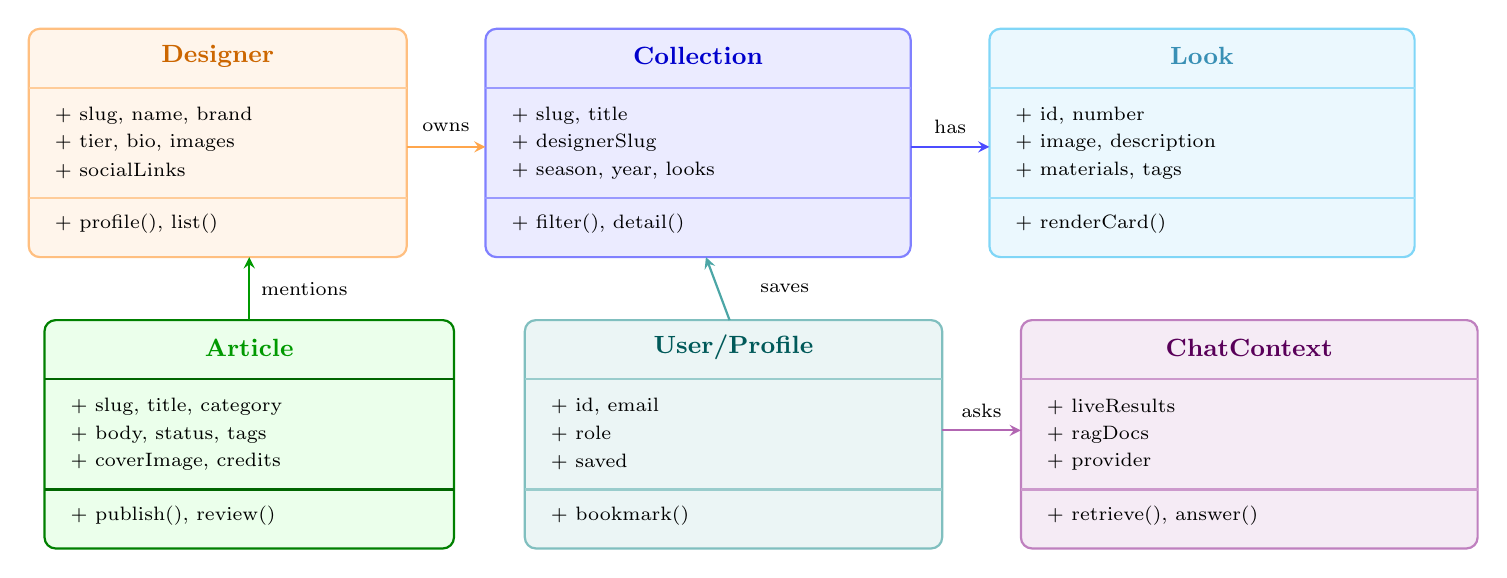
\begin{tikzpicture}[x=1cm,y=1cm,>=stealth,thick]
  % Designer
  \draw[rounded corners=4pt, fill=orange!8, draw=orange!50] (0,6.4) rectangle (4.8,9.3);
  \node[font=\small\bfseries, text=orange!80!black] at (2.4,8.95) {Designer};
  \draw[orange!40] (0,8.55) -- (4.8,8.55);
  \node[anchor=west,font=\scriptsize] at (0.2,8.20) {+ slug, name, brand};
  \node[anchor=west,font=\scriptsize] at (0.2,7.85) {+ tier, bio, images};
  \node[anchor=west,font=\scriptsize] at (0.2,7.50) {+ socialLinks};
  \draw[orange!40] (0,7.15) -- (4.8,7.15);
  \node[anchor=west,font=\scriptsize] at (0.2,6.82) {+ profile(), list()};

  % Collection
  \draw[rounded corners=4pt, fill=blue!8, draw=blue!50] (5.8,6.4) rectangle (11.2,9.3);
  \node[font=\small\bfseries, text=blue!80!black] at (8.5,8.95) {Collection};
  \draw[blue!40] (5.8,8.55) -- (11.2,8.55);
  \node[anchor=west,font=\scriptsize] at (6.0,8.20) {+ slug, title};
  \node[anchor=west,font=\scriptsize] at (6.0,7.85) {+ designerSlug};
  \node[anchor=west,font=\scriptsize] at (6.0,7.50) {+ season, year, looks};
  \draw[blue!40] (5.8,7.15) -- (11.2,7.15);
  \node[anchor=west,font=\scriptsize] at (6.0,6.82) {+ filter(), detail()};

  % Look
  \draw[rounded corners=4pt, fill=cyan!8, draw=cyan!50] (12.2,6.4) rectangle (17.6,9.3);
  \node[font=\small\bfseries, text=cyan!70!black] at (14.9,8.95) {Look};
  \draw[cyan!40] (12.2,8.55) -- (17.6,8.55);
  \node[anchor=west,font=\scriptsize] at (12.4,8.20) {+ id, number};
  \node[anchor=west,font=\scriptsize] at (12.4,7.85) {+ image, description};
  \node[anchor=west,font=\scriptsize] at (12.4,7.50) {+ materials, tags};
  \draw[cyan!40] (12.2,7.15) -- (17.6,7.15);
  \node[anchor=west,font=\scriptsize] at (12.4,6.82) {+ renderCard()};

  % Article
  \draw[rounded corners=4pt, fill=green!8, draw=green!50!black] (0.2,2.7) rectangle (5.4,5.6);
  \node[font=\small\bfseries, text=green!60!black] at (2.8,5.25) {Article};
  \draw[green!40!black] (0.2,4.85) -- (5.4,4.85);
  \node[anchor=west,font=\scriptsize] at (0.4,4.50) {+ slug, title, category};
  \node[anchor=west,font=\scriptsize] at (0.4,4.15) {+ body, status, tags};
  \node[anchor=west,font=\scriptsize] at (0.4,3.80) {+ coverImage, credits};
  \draw[green!40!black] (0.2,3.45) -- (5.4,3.45);
  \node[anchor=west,font=\scriptsize] at (0.4,3.12) {+ publish(), review()};

  % User/Profile
  \draw[rounded corners=4pt, fill=teal!8, draw=teal!50] (6.3,2.7) rectangle (11.6,5.6);
  \node[font=\small\bfseries, text=teal!70!black] at (8.95,5.25) {User/Profile};
  \draw[teal!40] (6.3,4.85) -- (11.6,4.85);
  \node[anchor=west,font=\scriptsize] at (6.5,4.50) {+ id, email};
  \node[anchor=west,font=\scriptsize] at (6.5,4.15) {+ role};
  \node[anchor=west,font=\scriptsize] at (6.5,3.80) {+ saved};
  \draw[teal!40] (6.3,3.45) -- (11.6,3.45);
  \node[anchor=west,font=\scriptsize] at (6.5,3.12) {+ bookmark()};

  % ChatContext
  \draw[rounded corners=4pt, fill=violet!8, draw=violet!50] (12.6,2.7) rectangle (18.4,5.6);
  \node[font=\small\bfseries, text=violet!70!black] at (15.5,5.25) {ChatContext};
  \draw[violet!40] (12.6,4.85) -- (18.4,4.85);
  \node[anchor=west,font=\scriptsize] at (12.8,4.50) {+ liveResults};
  \node[anchor=west,font=\scriptsize] at (12.8,4.15) {+ ragDocs};
  \node[anchor=west,font=\scriptsize] at (12.8,3.80) {+ provider};
  \draw[violet!40] (12.6,3.45) -- (18.4,3.45);
  \node[anchor=west,font=\scriptsize] at (12.8,3.12) {+ retrieve(), answer()};

  % Relationships
  \draw[->, orange!70] (4.8,7.8) -- (5.8,7.8);
  \node[font=\scriptsize, fill=white, inner sep=1pt] at (5.3,8.05) {owns};
  \draw[->, blue!70] (11.2,7.8) -- (12.2,7.8);
  \node[font=\scriptsize, fill=white, inner sep=1pt] at (11.7,8.05) {has};
  \draw[->, green!60!black] (2.8,5.6) -- (2.8,6.4);
  \node[font=\scriptsize, fill=white, inner sep=1pt] at (3.5,6.0) {mentions};
  \draw[->, teal!70] (8.9,5.6) -- (8.6,6.4);
  \node[font=\scriptsize, fill=white, inner sep=1pt] at (9.6,6.0) {saves};
  \draw[->, violet!60] (11.6,4.2) -- (12.6,4.2);
  \node[font=\scriptsize, fill=white, inner sep=1pt] at (12.1,4.45) {asks};
\end{tikzpicture}
}
  \caption[Платформын дотоод класс бүтэц]{Платформын дотоод класс ба domain object-ийн бүтэц}
  \label{fig:internal-class-architecture}
\end{figure}

Фронтэндээс нийтлэл авах урсгал дараах байдлаар явагдана: page/component нь content client helper дуудаж, helper нь public API route руу хүсэлт илгээж, API route нь repository method ашиглан CouchDB document уншаад фронтэндэд domain object хэлбэрээр буцаана. Admin талд ижил урсгал ажиллах боловч API route нь эхлээд Supabase session болон role шалгана.

\section{API зохиомж}
API зохиомж нь public унших API, хамгаалагдсан admin API, медиа файлын API, chat API гэсэн бүлэгтэй. Public API нь зөвхөн published content уншихад зориулагдана. Admin API нь editor/admin role-той хэрэглэгч нийтлэл, коллекц, дизайнер, медиа файл удирдахад хэрэглэгдэнэ. Харин хэрэглэгч урих болон эрх өөрчлөх API нь зөвхөн admin role-той хэрэглэгчид нээлттэй байна. Chat API нь архивын контекст болон RAG document ашиглан AI хариулт үүсгэнэ.

{\small
\begin{longtable}{|L{0.29\textwidth}|L{0.16\textwidth}|L{0.31\textwidth}|L{0.14\textwidth}|}
  \hline
  \textbf{API} & \textbf{Method} & \textbf{Үүрэг} & \textbf{Access} \\ \hline
  \path{/api/content/articles} & GET & Published article жагсаалт авах & Public \\ \hline
  \path{/api/content/articles/[slug]} & GET & Нэг нийтлэлийн detail авах & Public \\ \hline
  \path{/api/content/collections} & GET & Collection жагсаалт, filter авах & Public \\ \hline
  \path{/api/content/collections/[slug]} & GET & Collection detail ба looks авах & Public \\ \hline
  \path{/api/content/designers} & GET & Designer list авах & Public \\ \hline
  \path{/api/content/designers/[slug]} & GET & Designer profile авах & Public \\ \hline
  \path{/api/content/search-index} & GET & Global search-д хэрэгтэй index авах & Public \\ \hline
  \path{/api/admin/content/articles} & GET/POST & Нийтлэл жагсаах, шинээр үүсгэх & Editor/Admin \\ \hline
  \path{/api/admin/content/articles/[id]} & GET/PUT/DELETE & Нийтлэл detail авах, засах, устгах & Editor/Admin \\ \hline
  \path{/api/admin/content/collections} & GET/POST & Collection удирдах & Editor/Admin \\ \hline
  \path{/api/admin/content/designers} & GET/POST & Designer удирдах & Editor/Admin \\ \hline
  \path{/api/admin/content/assets} & GET/POST & Asset list болон upload хийх & Editor/Admin \\ \hline
  \path{/api/admin/invite} & POST & Багийн гишүүн урих, анхны эрх оноох & Admin \\ \hline
  \path{/api/admin/users/[id]/role} & PATCH & Хэрэглэгчийн эрх өөрчлөх & Admin \\ \hline
  \path{/api/profile/delete} & DELETE & Өөрийн profile, bookmark, auth user устгах & Auth \\ \hline
  \path{/api/content/assets/[id]/[name]} & GET & CouchDB attachment serve хийх & Public read \\ \hline
  \path{/api/chat} & POST & AI chatbot хариулт үүсгэх & Public/Auth \\ \hline
  \caption{API endpoint-ийн зохиомж}
  \label{tab:api-design}\\
\end{longtable}
}

Global search болон AI chatbot-ийн API урсгалыг дараах дарааллын диаграмуудаар харуулав. Search overlay нь search index дээр ranking хийж, chat API нь live content болон RAG context цуглуулан prompt бүрдүүлнэ.

\begin{figure}[htbp]
  \centering
  \resizebox{\textwidth}{!}{\begin{tikzpicture}[x=1cm,y=1cm,>=stealth,thick]
  \tikzstyle{box}=[draw, rounded corners=4pt, minimum width=2.55cm, minimum height=0.8cm,
    text width=2.35cm, align=center, font=\scriptsize]
  \tikzstyle{msg}=[font=\scriptsize, fill=white, inner sep=1pt, text width=3.1cm, align=center]

  \node[box] (u) at (0,0) {Хэрэглэгч};
  \node[box] (ui) at (4,0) {Search UI};
  \node[box] (engine) at (8.5,0) {Ranking\\engine};
  \node[box] (db) at (12.7,0) {Search\\index API};

  \draw[dashed] (0,-0.5) -- (0,-8.2);
  \draw[dashed] (4,-0.5) -- (4,-8.2);
  \draw[dashed] (8.5,-0.5) -- (8.5,-8.2);
  \draw[dashed] (12.7,-0.5) -- (12.7,-8.2);

  \draw[->] (0,-1.2) -- (4,-1.2);
  \node[msg, above] at (2,-1.2) {1. Search нээх};
  \draw[->] (4,-2.2) -- (12.7,-2.2);
  \node[msg, above] at (8.35,-2.2) {2. Index API дуудах};
  \draw[->] (12.7,-3.2) -- (4,-3.2);
  \node[msg, above] at (8.35,-3.2) {3. Нэгтгэсэн index};
  \draw[->] (4,-4.2) -- (0,-4.2);
  \node[msg, above] at (2,-4.2) {4. Query авах};
  \draw[->] (0,-5.2) -- (8.5,-5.2);
  \node[msg, above] at (4.25,-5.2) {5. Query ба filter};
  \draw[->] (8.5,-6.2) -- (12.7,-6.2);
  \node[msg, above] at (10.6,-6.2) {6. Оноо тооцох};
  \draw[->] (12.7,-7.2) -- (4,-7.2);
  \node[msg, above] at (8.35,-7.2) {7. Ангилсан result};
  \draw[->] (4,-7.8) -- (0,-7.8);
  \node[msg, above] at (2,-7.8) {8. Result сонгох};
\end{tikzpicture}
}
  \caption[Global search API урсгал]{Global search overlay ба search index API-ийн урсгал}
  \label{fig:api-search-sequence}
\end{figure}

\begin{figure}[htbp]
  \centering
  \resizebox{\textwidth}{!}{\begin{tikzpicture}[x=1cm,y=1cm,>=stealth,thick]
  \tikzstyle{box}=[draw, rounded corners=4pt, minimum width=2.55cm, minimum height=0.8cm,
    text width=2.35cm, align=center, font=\scriptsize]
  \tikzstyle{msg}=[font=\scriptsize, fill=white, inner sep=1pt, text width=3.0cm, align=center]

  \node[box] (u) at (0,0) {Хэрэглэгч};
  \node[box] (ui) at (4.0,0) {Chat UI};
  \node[box] (api) at (8.0,0) {Chat API};
  \node[box] (rag) at (12.0,0) {Live/RAG\\context};
  \node[box] (llm) at (16.0,0) {Gemini\\Ollama};

  \draw[dashed] (0,-0.5) -- (0,-8.2);
  \draw[dashed] (4.0,-0.5) -- (4.0,-8.2);
  \draw[dashed] (8.0,-0.5) -- (8.0,-8.2);
  \draw[dashed] (12.0,-0.5) -- (12.0,-8.2);
  \draw[dashed] (16.0,-0.5) -- (16.0,-8.2);

  \draw[->] (0,-1.2) -- (4.0,-1.2);
  \node[msg, above] at (2.0,-1.2) {1. Асуулт бичих};
  \draw[->] (4.0,-2.1) -- (8.0,-2.1);
  \node[msg, above] at (6.0,-2.1) {2. Message илгээх};
  \draw[->] (8.0,-3.0) -- (12.0,-3.0);
  \node[msg, above] at (10.0,-3.0) {3. Context хайх};
  \draw[->] (12.0,-3.9) -- (8.0,-3.9);
  \node[msg, above] at (10.0,-3.9) {4. Холбоотой эх сурвалж};
  \draw[->] (8.0,-4.8) -- (16.0,-4.8);
  \node[msg, above] at (12.0,-4.8) {5. Prompt ба context};
  \draw[->] (16.0,-5.8) -- (8.0,-5.8);
  \node[msg, above] at (12.0,-5.8) {6. Архивт тулгуурласан хариу};
  \draw[->] (8.0,-6.8) -- (4.0,-6.8);
  \node[msg, above] at (6.0,-6.8) {7. Хариу ба source};
  \draw[->] (4.0,-7.6) -- (0,-7.6);
  \node[msg, above] at (2.0,-7.6) {8. Хариулт унших};
\end{tikzpicture}
}
  \caption[AI chatbot API урсгал]{AI chatbot API, live archive, RAG context-ийн урсгал}
  \label{fig:api-chat-sequence}
\end{figure}

\section{Өгөгдлийн сангийн зохиомж}
Өгөгдлийн сангийн зохиомж нь content document болон user/auth relational өгөгдлийг хослуулсан hybrid загвартай. Загварын сэтгүүлийн content нь талбарын хувьд уян хатан тул article, collection, designer, asset-ийг CouchDB document байдлаар хадгална. Харин хэрэглэгчийн session, role, bookmark, RAG index зэрэг owner болон query policy шаарддаг өгөгдлийг Supabase/PostgreSQL-д хадгална.

\begin{figure}[htbp]
  \centering
  \resizebox{\textwidth}{!}{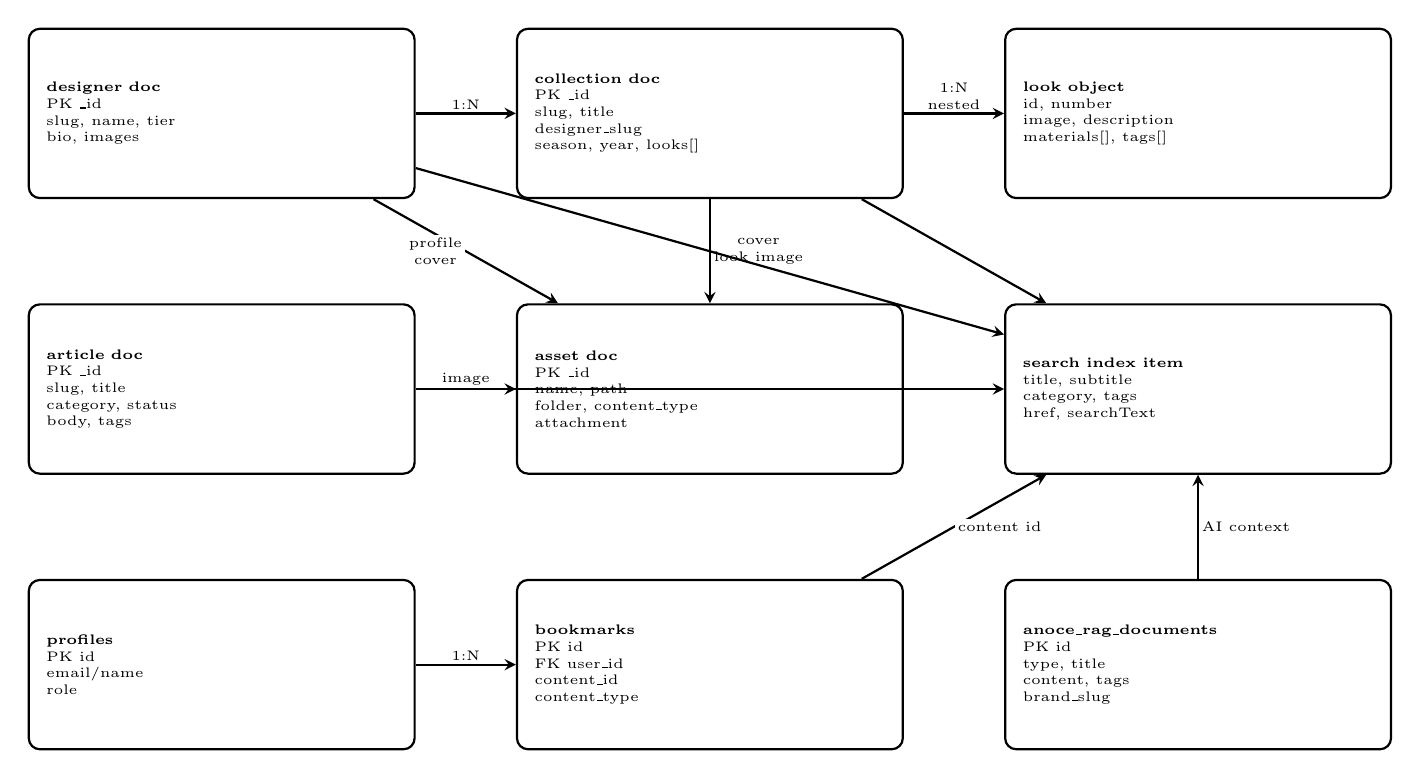
\begin{tikzpicture}[x=1cm,y=1cm,>=stealth,thick]
  \tikzstyle{entity}=[draw, rounded corners=4pt, minimum width=4.9cm, minimum height=2.15cm,
    text width=4.45cm, align=left, font=\tiny]
  \tikzstyle{rel}=[font=\tiny, fill=white, inner sep=1pt, align=center]

  \node[entity] (designer) at (0,6.6) {\textbf{designer doc}\\PK \_id\\slug, name, tier\\bio, images};
  \node[entity] (collection) at (6.2,6.6) {\textbf{collection doc}\\PK \_id\\slug, title\\designer\_slug\\season, year, looks[]};
  \node[entity] (look) at (12.4,6.6) {\textbf{look object}\\id, number\\image, description\\materials[], tags[]};

  \node[entity] (article) at (0,3.1) {\textbf{article doc}\\PK \_id\\slug, title\\category, status\\body, tags};
  \node[entity] (asset) at (6.2,3.1) {\textbf{asset doc}\\PK \_id\\name, path\\folder, content\_type\\attachment};
  \node[entity] (search) at (12.4,3.1) {\textbf{search index item}\\title, subtitle\\category, tags\\href, searchText};

  \node[entity] (profile) at (0,-0.4) {\textbf{profiles}\\PK id\\email/name\\role};
  \node[entity] (bookmark) at (6.2,-0.4) {\textbf{bookmarks}\\PK id\\FK user\_id\\content\_id\\content\_type};
  \node[entity] (rag) at (12.4,-0.4) {\textbf{anoce\_rag\_documents}\\PK id\\type, title\\content, tags\\brand\_slug};

  \draw[->] (designer) -- node[above,rel] {1:N} (collection);
  \draw[->] (collection) -- node[above,rel] {1:N\\nested} (look);
  \draw[->] (article) -- node[above,rel] {image} (asset);
  \draw[->] (collection) -- node[right,rel] {cover\\look image} (asset);
  \draw[->] (designer) -- node[left,rel] {profile\\cover} (asset);
  \draw[->] (designer) -- (search);
  \draw[->] (collection) -- (search);
  \draw[->] (article) -- (search);
  \draw[->] (profile) -- node[above,rel] {1:N} (bookmark);
  \draw[->] (bookmark) -- node[right,rel] {content id} (search);
  \draw[->] (rag) -- node[right,rel] {AI context} (search);
\end{tikzpicture}
}
  \caption[Өгөгдлийн сангийн ER/document зохиомж]{Өгөгдлийн сангийн ER/document зохиомж}
  \label{fig:database-design-er}
\end{figure}

{\small
\begin{longtable}{|L{0.18\textwidth}|L{0.24\textwidth}|L{0.08\textwidth}|L{0.20\textwidth}|L{0.18\textwidth}|}
  \hline
  \textbf{Хүснэгт/document} & \textbf{Гол талбар} & \textbf{PK} & \textbf{FK/Relation} & \textbf{Тайлбар} \\ \hline
  designer doc & \_id, slug, name, tier, bio, images & \_id & collection.designer\_slug & Дизайнерын profile мэдээлэл \\ \hline
  collection doc & \_id, slug, title, season, year, looks[] & \_id & designer\_slug & Коллекц болон nested look \\ \hline
  article doc & \_id, slug, title, category, status, body, tags & \_id & designer slug, asset path & Editorial нийтлэл \\ \hline
  asset doc & \_id, name, path, folder, content\_type, size & \_id & article/collection image & Зураг болон attachment metadata \\ \hline
  profiles & id, email, name, role, avatar\_url & id & auth.users.id & Хэрэглэгчийн role ба profile \\ \hline
  bookmarks & id, user\_id, content\_id, content\_type & id & profiles.id & Хэрэглэгчийн хадгалсан content \\ \hline
  anoce\_rag\_documents & id, title, content, category, tags, source & id & brand/content slug & AI chatbot-ийн retrieval context \\ \hline
  \caption{Өгөгдлийн сангийн хүснэгт/document зохиомж}
  \label{tab:database-table-design}\\
\end{longtable}
}

CouchDB document бүр stable \texttt{\_id}, \texttt{\_rev}, \texttt{type}, \texttt{slug}, \texttt{created\_at}, \texttt{updated\_at} metadata-тай байх ёстой. Repository layer нь update хийх үед өмнөх revision хадгалж conflict эрсдэлийг бууруулна. Supabase талд profile role болон bookmark owner-ийн policy тодорхой байх шаардлагатай.

\section{UI/UX зохиомж}
UI/UX зохиомжийн гол зарчим нь загварын сэтгүүлийн visual-first шинжийг хадгалах, гэхдээ admin болон archive workflow-г ойлгомжтой, дахин ашиглахад хялбар болгох явдал юм. Public тал editorial, archive, designer directory, collection detail, article detail, search overlay, profile, journal, careers, press гэсэн үндсэн navigation-тай байна. Admin тал dashboard, articles, collections, designers, assets, calendar гэсэн бүтэцтэй бөгөөд users хэсэг зөвхөн админд харагдана.

\begin{table}[htbp]
  \centering
  \small
  \begin{tabular}{|L{0.22\textwidth}|L{0.34\textwidth}|L{0.30\textwidth}|}
    \hline
    \textbf{Хэсэг} & \textbf{Navigation} & \textbf{UX зорилго} \\ \hline
    Public site & Home, Archive, Designers, Editorial, Journal, Careers, Press, Search, Login/Profile & Уншигч контент хурдан олох \\ \hline
    Article detail & Title, cover image, body, tag, related looks & Сэтгүүлийн унших туршлага бүрдүүлэх \\ \hline
    Collection detail & Hero image, designer, season/year, look gallery, materials & Зурагт archive-ийг ойлгомжтой үзүүлэх \\ \hline
    Search overlay & Query input, grouped result, recent search, season filter & Олон entity-г нэг дор хайх \\ \hline
    Admin CMS & Dashboard, Articles, Collections, Designers, Assets, Calendar, Users & Контент удирдах ажлыг төвлөрүүлэх; Users хэсгийг зөвхөн админд харуулах \\ \hline
  \end{tabular}
\vspace{0.4em}
  \caption{Навигацийн бүтэц}
  \label{tab:navigation-structure}
\end{table}

Responsive layout-д card grid, image ratio, filter bar, table overflow, button label, form field, modal/overlay зэрэг элементүүд viewport өөрчлөгдөхөд давхцахгүй байх шаардлагатай. Public тал зураг том, текст богино, scan хийхэд хялбар байх ёстой бол admin тал мэдээлэл нягт боловч эмхтэй, form label болон status badge ойлгомжтой байх ёстой.

\section{Аюулгүй байдлын зохиомж}
Аюулгүй байдлын зохиомж нь authentication, authorization, protected route, input validation, upload validation, secret management, AI context boundary гэсэн чиглэлтэй. Client дээр admin link нуух нь хангалтгүй тул server-side API route бүр role шалгах шаардлагатай. Password authentication болон session management-д Supabase Auth ашиглана.

\begin{longtable}{|L{0.22\textwidth}|L{0.34\textwidth}|L{0.30\textwidth}|}
  \hline
  \textbf{Хамгаалалт} & \textbf{Зохиомж} & \textbf{Хэрэглэх хэсэг} \\ \hline
  Password/session & Supabase Auth ашиглан session удирдах & Login, profile, admin access \\ \hline
  Role-based access control & admin/editor/reader role шалгах & Admin route, admin API \\ \hline
  Admin-only user management & Хэрэглэгч урих, эрх өөрчлөх үйлдлийг зөвхөн админд нээх & \path{/admin/users}, invite/role API \\ \hline
  Protected API & Unauthorized үед 401, forbidden үед 403 буцаах & \path{/api/admin/content/*} \\ \hline
  Input validation & Required field, slug, status, category шалгах & Article/collection/designer form \\ \hline
  Upload validation & File type, size, folder metadata хянах & Asset upload \\ \hline
  Secret management & Provider key, DB credential-ийг server-side env-д хадгалах & Chat API, CouchDB, Supabase service \\ \hline
  AI grounding & Live/RAG context байхгүй үед зохиомол баримт өгөхгүй байх & Chatbot prompt/fallback \\ \hline
  \caption{Аюулгүй байдлын зохиомж}
  \label{tab:security-design}\\
\end{longtable}

\section{Ашигласан технологийн сонголт}
Технологийн сонголтыг фронтэнд, бэкенд/API, өгөгдлийн сан, нэвтрэлт танилт, загварчлал, AI, байршуулах орчин гэсэн давхаргаар авч үзэв. Next.js нь App Router, dynamic route, API route, server/client component зэрэг боломжтой тул нэг codebase дотор public site, admin CMS, backend API-г зохион байгуулахад тохиромжтой \cite{nextjs_docs}. React component-based UI-д, TypeScript typed domain model-д, Tailwind CSS responsive layout-д, CouchDB уян JSON document store-д, Supabase auth/role/bookmark/RAG layer-д, RAG арга AI context grounding-д ашиглагдана \cite{react_learn,tailwind_docs,couchdb_docs,supabase_docs,rag_lewis_2020}.

\begin{longtable}{|L{0.17\textwidth}|L{0.25\textwidth}|L{0.33\textwidth}|L{0.15\textwidth}|}
  \hline
  \textbf{Давхарга} & \textbf{Технологи} & \textbf{Сонгосон шалтгаан} & \textbf{Төлөв} \\ \hline
  Фронтэнд & Next.js, React, TypeScript & Component-based, typed, route зохион байгуулалт сайн & Хэрэгжсэн \\ \hline
  Styling/UI & Tailwind CSS, Framer Motion & Responsive visual archive, animation, хурдан prototype & Хэрэгжсэн \\ \hline
  Бэкенд/API & Next.js API routes & Public/admin/chat API-г нэг codebase-д байрлуулах & Хэрэгжсэн \\ \hline
  Контентын өгөгдлийн сан & CouchDB & Article, collection, designer, asset JSON document уян хадгалах & Хэрэгжсэн \\ \hline
  Auth/user data & Supabase & Auth, profile role, bookmark, RAG index хурдан хэрэгжүүлэх & Хэрэгжсэн \\ \hline
  Хайлт & Client lexical scoring + search index API & MVP-д хурдан, ойлгомжтой, өргөтгөх боломжтой & Хэрэгжсэн \\ \hline
  AI & RAG + Gemini/Ollama fallback & Archive context-д тулгуурласан хариулт, provider уян хатан & Хэрэгжсэн \\ \hline
  Байршуулах орчин & Vercel/Render/Supabase managed services & Deploy хийхэд хялбар, managed backend ашиглах боломжтой & Төлөвлөсөн \\ \hline
  \caption{Ашигласан технологийн сонголт}
  \label{tab:technology-choice}\\
\end{longtable}

\section{Бүлгийн дүгнэлт}
Гуравдугаар бүлгээр платформыг хэрхэн байгуулахыг архитектур, дотоод бүтэц, API, өгөгдлийн сан, UI/UX, аюулгүй байдал, технологийн сонголтын түвшинд тодорхойлов. Энэхүү зохиомж нь хоёрдугаар бүлгийн шаардлагыг хэрэгжилттэй холбох гүүр болж, дараагийн бүлэгт бодит frontend, backend, database, authentication, туршилтын үр дүнг тайлбарлах суурь болно.
